\section{Differentiable Digital Signal Processing}
\label{section:DDSP}

Differentiable Digital Signal Processors (DDSP) are differentiable versions of traditional digital signal processing elements (such as harmonic oscillators and filtered noise banks) that can be integrated into machine learning models\cite{OriginalDDSP}. They are a relatively novel invention but build on the foundations of traditional spectral encoding and modelling techniques such as Mel-Spectrograms and Fourier transforms. Although they were designed to model musical instruments, they can be extended to the human voice.

The DDSP network is modular and consists of multiple separate feedforward components (featuring a separate encoder and decoder) instead of a single recurrent based network. Information is fed between the encoder and decoder in time-dependent information called latents; these are fundamental frequency and loudness.

The model aims to take advantage of what the authors call inductive biases of sound instead of making the model figure out all the features of sound itself. This idea is well validated and is known as the harmonic plus noise model of spectral modelling synthesis\cite{HarmonicPlusNoise}. For example, an instrument's track could have harmonic vibrations at multiples of the fundamental frequency and noise components coming from a white noise source through a series of filter banks that change over time.

\subsection{Spectral Modelling Synthesis}

DDSP synthesiser elements are based on traditional synthesiser-based components that can be combined with an encoder and decoder to form a complete machine learning model. DDSP uses a type of sound modelling called Spectral Modelling Synthesis\cite{SpectralModellingSynthesis} to model sound, with the components being modified, so they are differentiable. By recreating them as differentiable components, the gradients of each block can be accessed in the machine learning model, enabling them to be configured by the model. Synthesisers take the network outputs of the decoder and use them to synthesise an output audio signal.

\subsubsection{Harmonic Oscilator}

The harmonic oscillator is the first of the 2 Spectral Modelling Synthesis components. It consists of a bank of oscillators that output a sinusoidal signal denoted as $x(n)$ where $n$ represents discrete time steps and is equal to the sum of the sinusoidal waves. The harmonic oscillator can be expressed as:
\
\begin{equation}
    x(n) = \sum_{k=1}^{N} A_k(n) \sin(\phi_k(n))
\end{equation}

\begin{itemize}
    \item $x(n)$ is the output signal
    \item $A_k(n)$ is the amplitude of the kth sinusoidal oscillator
    \item $\phi_k(n)$ is the instantaneous phase of the kth sinusoidal oscillator
\end{itemize}

The phase at a certain point in the output signal can be calculated as follows using the instantaneous frequency:

\begin{equation}
    \phi(n) = 2\pi\sum_{m=0}^N f_k(m) + \phi_{0,k}
\end{equation}

\begin{itemize}
    \item $\phi_k(n)$ is the instantaneous phase of the kth sinusoidal oscillator
    \item $f_k(m)$ is the instantaneous frequency of the kth sinusoidal oscillator
    \item $\phi_0(k)$ is the initial phase of the kth sinusoidal oscillator
\end{itemize}

Like actual sound, each harmonic oscillator's frequency $f_k(m)$ is an integer multiple of the fundamental frequency $f_0(n)$. For example the kth harmonic oscillator, the instantaneous frequency is defined as:

\begin{equation}
    f_k(m) = k \times f_0(n)
\end{equation}

The highest harmonic should be at the Nyquist frequency, which is half the sample rate or mathematically as:

\begin{equation}
    f_{Nyquist} = N \times f_0(n)
\end{equation}

Defining the highest harmonic in this way ensures that the harmonic oscillator can represent all of the possible signal ranges.

The initial phase $\phi_0(k)$ can be random, fixed or learned\cite{OriginalDDSP}.

The oscillators operate at the sample rate; however, the neural network is trained at a lower rate. DDSP employs bilinear interpolation to increase the sample rate from that of the neural network and smoothing to prevent artefacts.

\vspace{0.5cm}
\framebox[1.1\width]{
    \begin{minipage}{0.8\textwidth}
        Bilinear interpolation is a mathematical technique enabling the estimation of new values between existing discrete values that are the functions of two variables. In DDSP, it is used to increase the neural network's sample rate to that of the underlying audio signal.
    \end{minipage}
}
\vspace{0.5cm}

\subsubsection{Filtered Noise}

The filtered noise is a component of the DDSP synthesiser. For example, white noise is filtered by a \acrfull{LTI-FIR} to produce a noise signal. LTV-FIR filters are a type of filter that can vary over time, enabling different noise patterns to be generated at different time steps in the output signal.

Finite impulse response filters consist of mathematical impulse responses, meaning that the filter is of finite duration, enabling the filter to change and, over time, model different stochastic noises in the output signal.

As the filters are linear time-invariant, the noise filter can be characterised by its response to different frequencies of sinusoids, known as its frequency response. The filter is also independent of time.

It is worth noting that the noise filter is applied in the frequency domain; this is done to avoid phase distortion. Phase distortion occurs when a filter's phase response is not linear in the frequency domain. A lack of linearity in the filter domain can distort the filter's output, making synthesised sounds sound unrealistic.

The neural network was tasked with predicting frequency domain transfer functions of the filter for every frame of the output signal, denoted as $H_l$\cite{OriginalDDSP}.

For all notations with subscript l, l denotes that the values are for the lth frame of the output signal.

$H_l$ is in the frequency domain; it shows the filter's frequency response. Even though LTV-FIR filters are not linear time-variant, the network can vary the FIR filter over time, allowing the filter to change over time for modelling different noise patterns.

As linear time-invariant filters can be denoted by their impulse response, the frequency response of the filter can be denoted by its impulse response $h$, as shown below:

\begin{equation}
    H_l = \mathscr{F}^{-1}(h_l)
\end{equation}

\begin{itemize}
    \item $H_l$ is the frequency response of the filter in the frequency domain
    \item $h$ is the impulse response of the filter
    \item $\mathscr{F}^{-1}$ is the inverse descrete Fourier transform
\end{itemize}

In order to apply the time-varying filter to map the input to the output, the following is done:

\begin{enumerate}
    \item An input white noise signal is split into non-overlapping frames of fixed hop size, each one to go with a certain impulse response $h_l$.
    \item Frames are then multiplied in the fourier domain: \begin{itemize}
        \item $Y_l = H_l X_l$
        \item $Y_l$ is the output signal, where $X_l = \mathscr{F}(x_l)$, where $\mathscr{F}$ is the \acrfull{DFT}
        \item $X_l$ is the input signal, where $Y_l = \mathscr{F}^{-1}(y_l)$, where $\mathscr{F}^{-1}$ is the \acrfull{IDFT}
    \end{itemize}
    \item Output audio frames are then retrieved using the inverse Fourier transform:
        $y_l = \mathscr{F}^{-1}(Y_l)$
    \item Output audio frames are then comnbined, using the same hop size as the input audio frames.
\end{enumerate}

\vspace{0.5cm}
\framebox[1.1\width]{
    \begin{minipage}{0.8\textwidth}
        Hop size refers to the number of samples between each frame; the number of samples in a frame equals the hop size.
    \end{minipage}
}
\vspace{0.5cm}

The filtered noise synthesiser can generate many different noise patterns that are not harmonic and continuous. The original DDSP authors used them to generate unique instrument features, such as the plucking of a violin, but they can also be used to generate consonants in the human voice \cite{SingingDDSP}.

\subsection{Model Setup}

\begin{figure}[!ht]
    \centering
    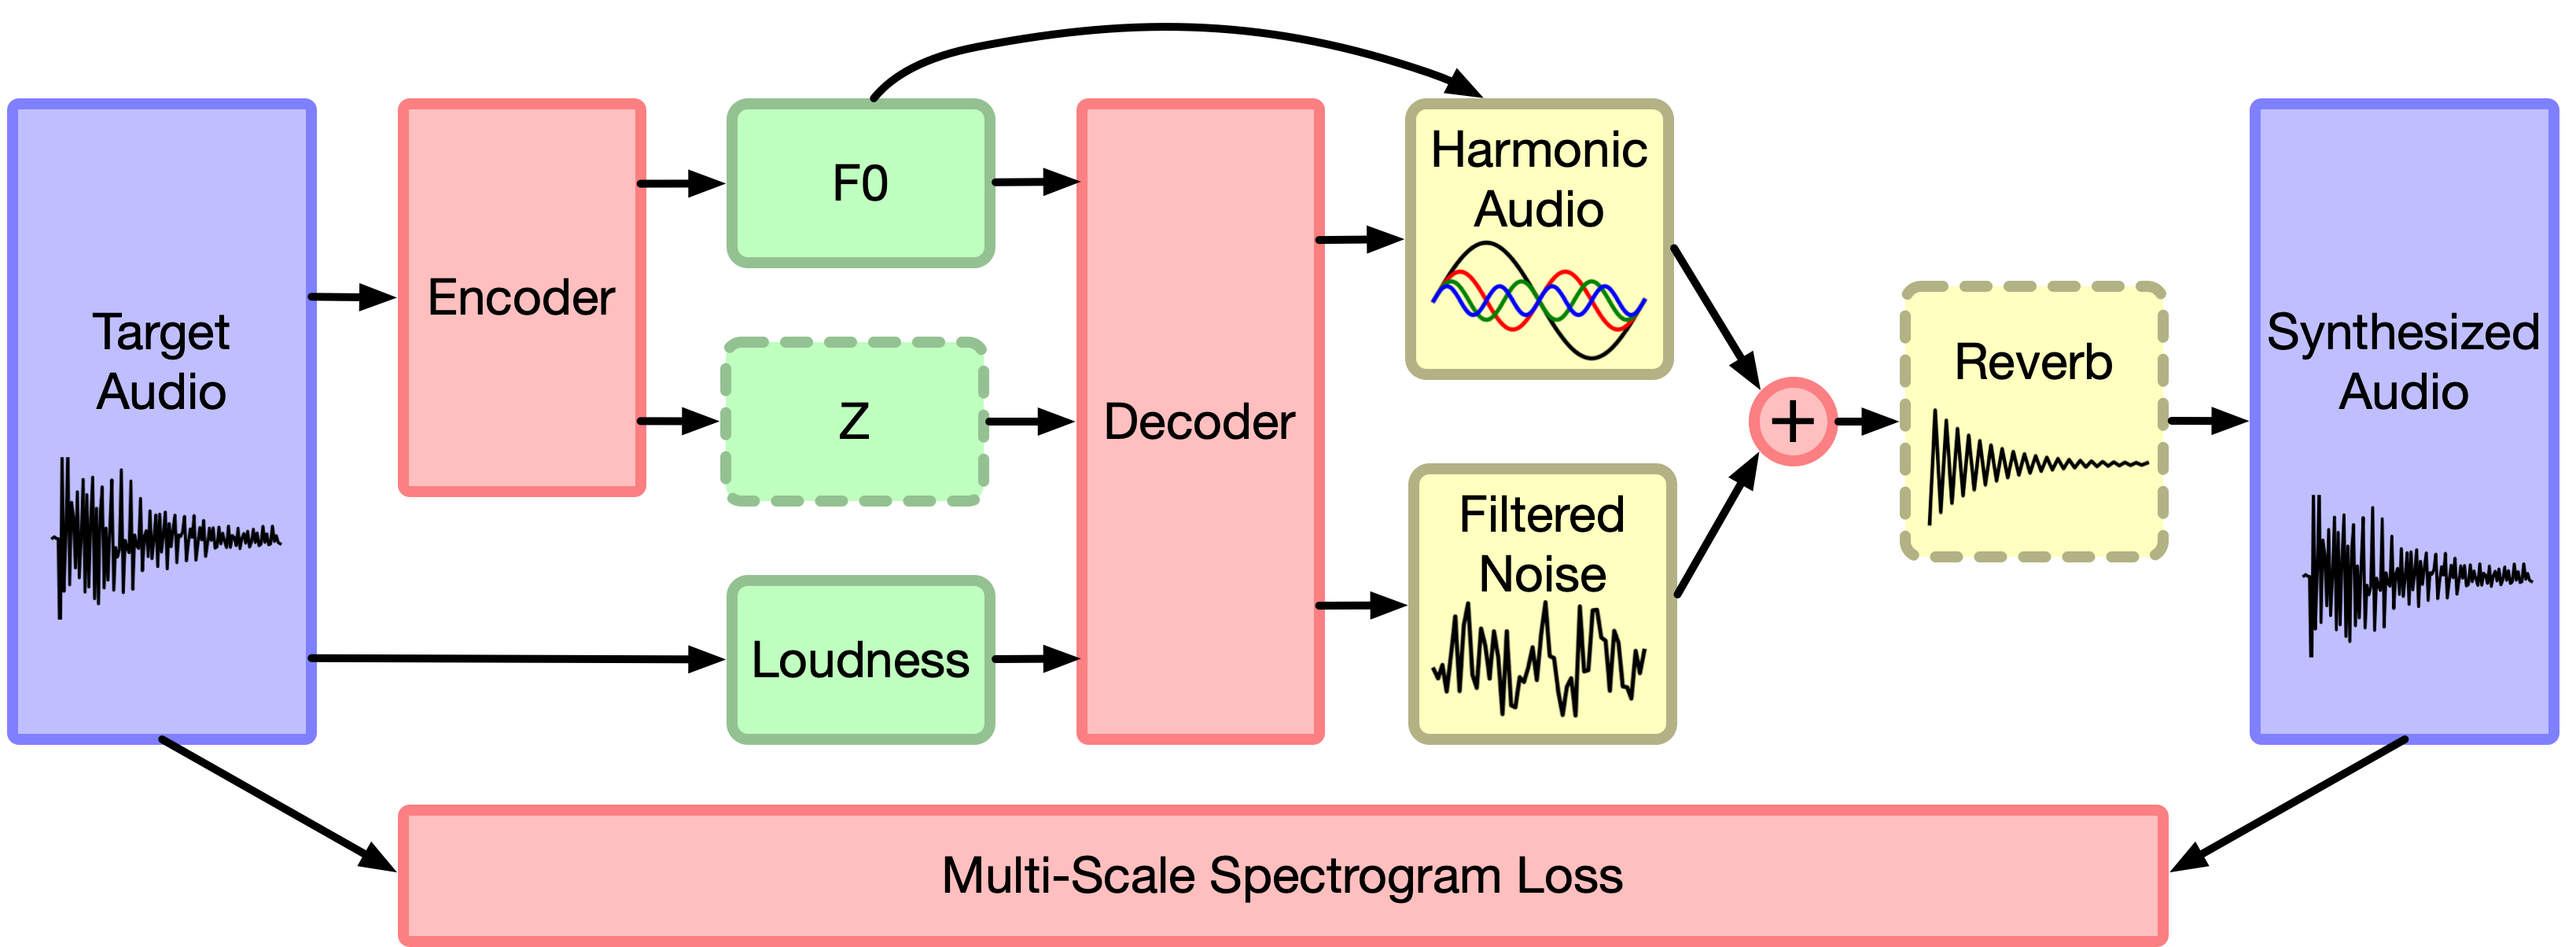
\includegraphics[width=0.8\textwidth]{literature_review/DDSPArchitecture.png}
    \caption{The DDSP Model Architecture: The model setup from the original paper\cite{OriginalDDSP} standardised machine learning components are shown in red, the latent varibles in green and the synthesizers in yellow.}
    \label{fig:ddsp_model_setup}
\end{figure}

The harmonic oscillators and filtered noise are combined to produce the synthesised output signal in what is known as the Harmonic plus Noise model. The combined output can also be passed through additional modules to produce different types of sounds, for example, a reverberation module to accurately model the acoustic characteristics of a string instrument; this is, however, beyond the scope of this paper.

The initial DDSP model\cite{OriginalDDSP} employed a modified autoencoder decoder setup where the autoencoder was trained to minimise reconstruction loss in an outputted synthesised audio. Training data is fed into the encoder in the form of Mel-spectrogram images. The autoencoder attempts to extract information from the input signal. Residual information (Z) and F0, the fundamental frequency, are extracted using an encoder in the standard model. Loudness is statistically determined outside of the encoder.

Because loudness can be statistically determined from a spectrogram, making an encoder learn this would be inefficient.

As all of these quantities are time-dependent, they can be denoted as such: $f(t), l(t), z(t)$.

However, the DSP architecture is very flexible; therefore, different variations of this autoencoder setup can be used. For example, instead of forcing the encoder to map F0, CREPE can be used to extract the F0 from the input signal.

\vspace{0.5cm}
\framebox[1.1\width]{
    \begin{minipage}{0.8\textwidth}
        CREPE is a highly accurate pitch detection based \acrfull{CNN}\cite{CREPE}. It can accurately predict pitch with an accuracy of over 99.9\%. In addition, it is a pre-trained model that can be used with the DDSP library to extract the pitch from the input signal accurately.
    \end{minipage}
}
\vspace{0.5cm}

The decoder then uses the F0, Z, and the statistically determined loudness to derive control values for the filtered noise and oscillator synthesisers, learning how to re-synthesise the target-audio track.

The fundamental frequency is, however, additionally fed directly into the synthesisers as it enables the model to respond to frequencies unseen during training\cite{SingingDDSP}.

Due to the modular design, certain features can be explicitly controlled, for example, room acoustics. Some networks would implicitly pick up room acoustics. This method may introduce unnecessary mode covering, increasing potential training time. The DDSP model explicitly defines room acoustics using a reverberation synthesiser (see Figure \ref{fig:ddsp_model_setup}).

\subsection{Measure of Loss}
\label{sec:loss_measure}

In order to train the model, it is necessary for a measure of loss to be defined. The autoencoder is tasked with minimising the reconstruction loss; this is the difference between the synthesised audio and the target audio. Unlike in a conventional autoencoder model, the loss cannot be defined pointwise as two waveforms may sound the same but have different pointwise characteristics. The loss function is therefore defined using a method called multi-scale spectral loss. The loss is defined as the sum of L1 differences and the L1 log difference between the target and synthesised magnitude spectrograms.

\vspace{0.5cm}
\framebox[1.1\width]{
    \begin{minipage}{0.8\textwidth}
        L1 loss is defined as the sum of the absolute differences\cite{L1Statistic}, the sum of the absolute differences between the magnitude spectrograms.
    \end{minipage}
}
\vspace{0.5cm}

\begin{equation}
    L_i = ||S_i - \hat{S_i}||_1 + ||\log{S_i} - \log\hat{S_i}||_1
\end{equation}

\begin{itemize}
    \item $L_i$ is the model loss FFT of size $i$
    \item $S_i$ is the target spectrogram with a given FFT of size $i$
    \item $\hat{S_i}$ is the synthesized spectrogram with a given FFT of size $i$
    \item $||S_i - \hat{S_i}||_1$ is the L1 difference between the target and synthesized spectrograms
    \item $||\log{S_i} - \log\hat{S_i}||_1$ is the L1 difference between the target and synthesized logarithmic Mel-spectrograms
\end{itemize}

The total loss is then equal to the sum of spectral losses for different FFT sizes:

\begin{equation}
    L = \sum_{i=1} L_i
\end{equation}

Where $i \in (4096, 2048, 1024, 512, 256, 128, 64)$

\subsection{Speech Synthesis Using DDSP}

Further research on top of DDSP relating to vocals has been done for speech synthesis, although not directly designed for music; the paper introduces a slightly different system that modifies the DDSP architecture to more closely match the human voice\cite{SpeechDDSP}. Instead of using an autoencoder, the network uses a series of convolutional neural networks.

The method yields highly accurate results (although it is still noticeable that the output has been synthesised). Timbre was accurately measured, though consonants still sounded off. Unfortunately, the code used for the model was not available for download, limiting the value of the paper as its findings could not be replicated. It could, in theory, be reversed engineered though this would take considerable time and effort and is, as such, beyond the scope of this project. It is also possible that the results were cherry-picked from the original as only a limited number of samples were available.

\subsection{Singing Voice Synthesis Using DDSP}
\label{sec:singing_voice_synthesis}

A new team has conducted attractive work building on top of the initial paper to produce singing voice synthesis\cite{SingingDDSP} specifically. This paper outlines how the DDSP model can be further altered to interpret better and learn how to model the human voice.

The adaptation involved adding \acrfull{MFCC} an additional time-varying form of encoding. The coefficients together make up a \acrfull{MFC}. A Mel-frequency cepstrum (MFC) represents the spectrum of a signal using a non-linear Mel frequency scale.

MFFCs have a long history of use in telecommunications and speech processing\cite{MFCCHistory}. Thus, the original authors hypothesised that this representation of the residual z information would more accurately model the non-linearity of the human voice, thus making a vocal synthesis model more accurate.

The modified decoder and MLP can be seen in Figure \ref{fig:singing_decoder_mlp}. An additional MLP layer has been added to the decoder to allow for the MFC to be learned.

\begin{figure}[!ht]
    \centering
    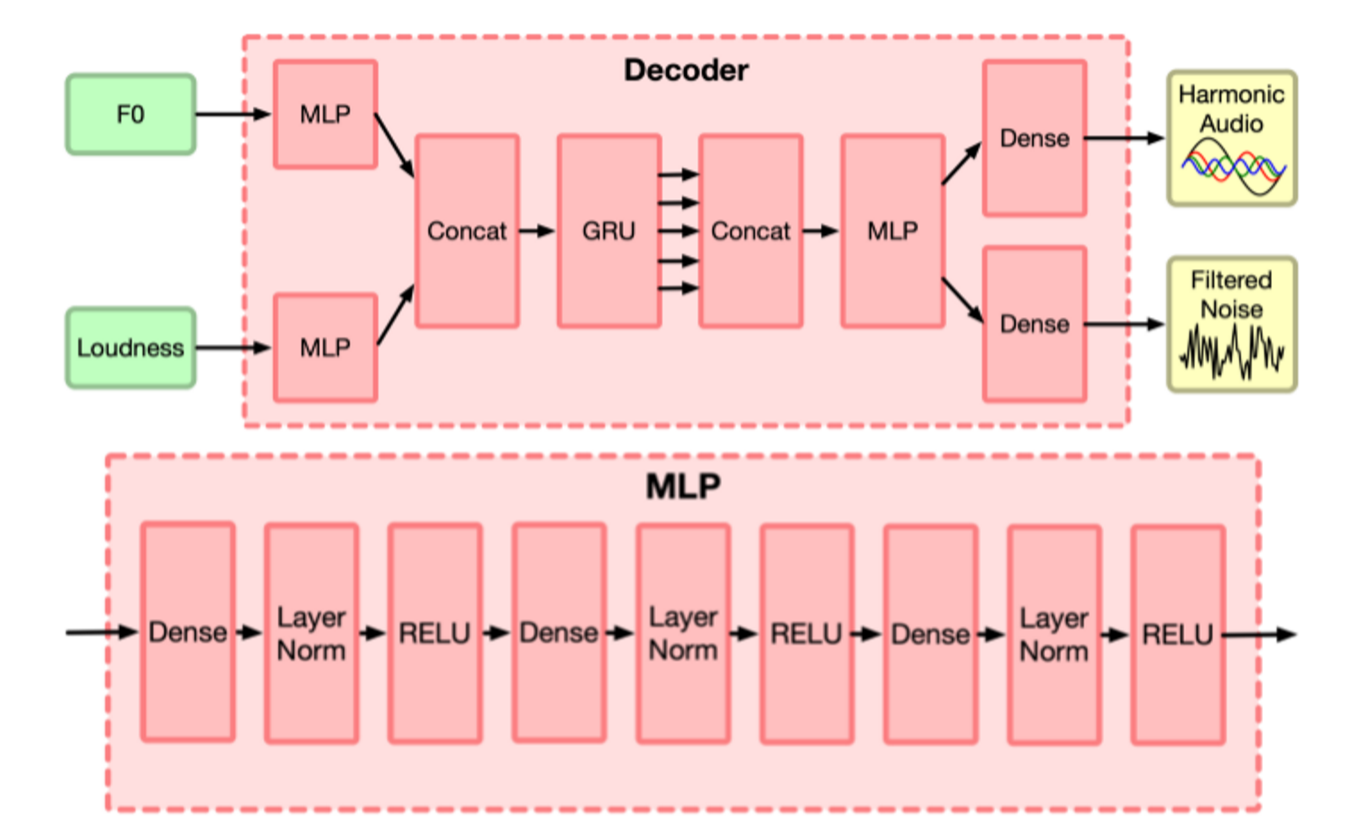
\includegraphics[width=0.8\textwidth]{literature_review/SingingDecoderMLP.png}
    \caption{Modified DDSP Decoder and MLP\cite{SingingDDSP}}
    \label{fig:singing_decoder_mlp}
\end{figure}

Even on a small dataset, promising results were obtained. Timbre transfer was possible. The performance of the modified decoder exceeded that of the original decoder.

Unfortunately, when the model was forced to recreate unseen sung lyrics, it was unintelligible, appearing to make stuttering noises. The model managed to obtain the correct loudness and pitch of the sound (except for the occasional pitch artefacts) but had no understanding of phonetics (i.e. the specific words that makeup speech). The paper suggests several steps for further work:

\begin{itemize}
    \item Phonetic condition of the model to model the nuances of human singing and to model the lyrics.
    \item Using synthesisers more suitable for modelling the human voice.
    \item Pre-processing of the fundamental frequency to remove pitch artefacts.
\end{itemize}

\subsection{DDSP Evaluation}

In the original paper, the DDSP decoder quickly learned how to re-synthesise datasets for a single instrument that sounded like the original audio sample.

A big pro of the method was that proper training on an instrument could be undertaken with as little as 15 minutes of training audio. Such a small dataset contrasts with models such as Jukebox, which require many hours of training audio as they are far larger models.

Due to the smaller model size, the model can operate with reduced training time and cost, making it more suitable for use in real-world applications and perhaps real-time applications.

Another plus was the interpretable and modular design of the model; individual factors such as timbre, pitch or loudness could be varied whilst keeping the others characteristics constant. This interpretation was possible because the model was conditioned to use pitch and loudness and the underlying residual z values to synthesise the audio.

Additionally, individual components can be changed, perhaps without rebuilding the whole model. E.g. the spectrum based encoder can be replaced with a midi sourced encoder, with the rest of the model architecture remaining unchanged.

It was eventually decided that using the DDSP model would be picked for further research due to its modularity, accuracy and ease of use.

The variation of DDSP designed for \nameref{sec:singing_voice_synthesis} was chosen as this is a relatively novel area of research and held the most exciting applicability. However, this has historically proven to be a complex problem to solve. The human voice is not a simple harmonic series with a constant timbre.